% Visual preamble adapted from slides_course/main.tex (2026-10-13).
\documentclass[aspectratio=169,12pt,t]{beamer}

% Speaker notes: uncomment ONE line to see them.
% \setbeameroption{show notes on second screen=right}  % dual-screen (pdfpc)
% \setbeameroption{show only notes}                     % notes handout

\usetheme[progressbar=none, sectionpage=none]{moloch}
% A 208 x 117 mm canvas retains 16:9 and the actual 12pt class fonts.
% Long owner-approved sentences fit without frame scaling or reduced fonts.
\geometry{paperwidth=208mm,paperheight=117mm}

% ---------- fonts ----------
\usepackage{fontspec}
\setsansfont{Avenir Next}[BoldFont={Avenir Next Demi Bold}]
\setmonofont{Menlo}[Scale=1.0]
\newcommand{\captiontype}{\small}

% ---------- palette ----------
\definecolor{navy}{HTML}{1F3A5F}
\definecolor{teal}{HTML}{2A9D8F}
\definecolor{fault}{HTML}{E76F51}
\definecolor{paper}{HTML}{FAFAF7}
\definecolor{ink}{HTML}{22262B}
\definecolor{muted}{HTML}{6B7280}
\definecolor{rule}{HTML}{D6D9DE}

\setbeamercolor{normal text}{fg=ink, bg=paper}
\setbeamercolor{frametitle}{fg=paper, bg=navy}
\setbeamercolor{progress bar}{fg=teal, bg=rule}
\setbeamercolor{alerted text}{fg=fault}
\setbeamercolor{example text}{fg=teal}
\setbeamercolor{structure}{fg=navy}
\setbeamercolor{title separator}{fg=teal}
\setbeamercolor{footline}{fg=muted}
% Beamer otherwise inherits the fault/alert color for in-slide citations.
\setbeamercolor{bibliography entry author}{fg=navy}
\setbeamercolor{bibliography entry title}{fg=ink}
\setbeamercolor{bibliography entry location}{fg=muted}
\setbeamercolor{bibliography entry note}{fg=muted}
\setbeamercolor{block title}{fg=paper, bg=navy}
\setbeamercolor{block body}{bg=navy!6}
\setbeamerfont{frametitle}{size=\large, series=\bfseries}
\setbeamertemplate{frametitle}{\nointerlineskip\begin{beamercolorbox}[wd=\paperwidth,sep=2mm,leftskip=4mm]{frametitle}\usebeamerfont{frametitle}\insertframetitle\strut\end{beamercolorbox}}
\setbeamertemplate{itemize items}{\color{teal}\rule[0.25ex]{0.45em}{0.45em}}
\setbeamertemplate{bibliography item}[text]
\setbeamertemplate{page number in head/foot}[totalframenumber]
\hypersetup{colorlinks=true, linkcolor=navy, urlcolor=navy, citecolor=navy}
% Keep the appendix bookmark free of Beamer translation commands.
\pdfstringdefDisableCommands{\def\translate#1{#1}}

\setbeamertemplate{itemize subitem}{\color{muted}--}

% ---------- packages ----------
\usepackage{tikz}
\usetikzlibrary{arrows.meta, positioning, automata, calc, shapes.geometric, fit, backgrounds, decorations.pathreplacing}
\usepackage{booktabs}
\usepackage{array}
\newcolumntype{L}[1]{>{\raggedright\arraybackslash}p{#1}}
\usepackage{amsmath}
\usepackage{siunitx}
\sisetup{detect-all}


\setbeamertemplate{navigation symbols}{}
\setbeamersize{text margin left=6mm,text margin right=6mm}
\setbeamertemplate{footline}{\hfill\color{muted}\small\insertframenumber/\inserttotalframenumber\hspace{6mm}\vspace{2mm}}
\linespread{1.10}
\newcommand{\src}[1]{\par\vfill{\small\color{muted}Source: #1}}
\newcommand{\takeaway}[1]{\par\medskip\begin{beamercolorbox}[sep=2mm,wd=\linewidth]{block body}\color{navy}\textbf{#1}\end{beamercolorbox}}
\begin{document}
\begin{frame}{Owner checkpoint | 13 October 2026}
\begin{itemize}
\item The Linux workload, UART protocol and FreeRTOS supervisor are implemented; inference is an OS workload.
\item Retained evidence covers Pi software timing, physical MCU transitions and analyzer captures, with explicit exclusions.
\item Immediate work: document the rig, verify the review fixes, restore clean power, then rerun under v2 rules.
\end{itemize}
\takeaway{The code is ahead of the clean physical evidence.}\src{P\_PROGRESS.md; results/README.md; docs/STAGE\_REPORT.md}
\end{frame}
\begin{frame}{System map | execution and ownership}

\centering
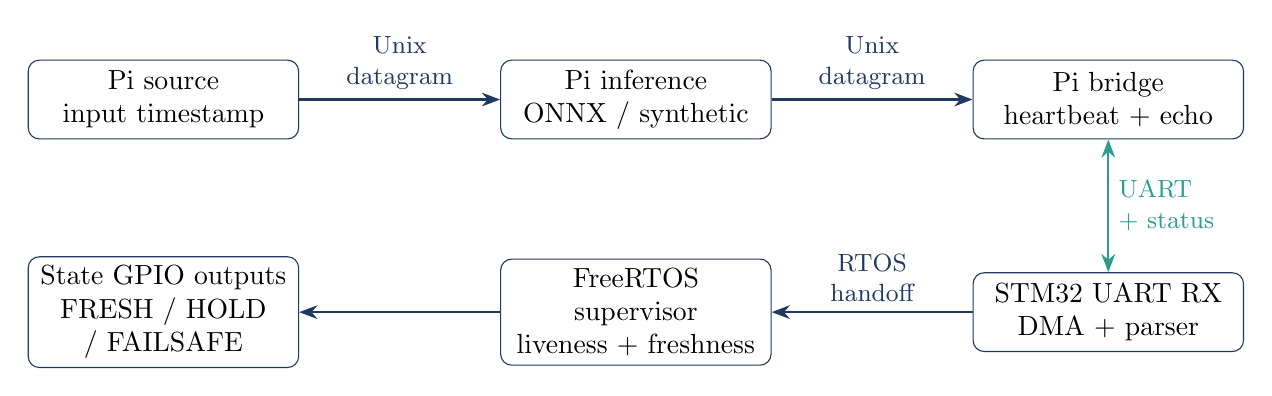
\begin{tikzpicture}[x=1cm,y=1cm,>=Stealth,box/.style={draw=navy,fill=white,rounded corners,align=center,text width=3.2cm,minimum height=1cm,font=\normalsize}]
\node[box] (s) at (0,0) {Pi source\\input timestamp};
\node[box] (i) at (6,0) {Pi inference\\ONNX / synthetic};
\node[box] (b) at (12,0) {Pi bridge\\heartbeat + echo};
\node[box] (m) at (12,-2.7) {STM32 UART RX\\DMA + parser};
\node[box] (u) at (6,-2.7) {FreeRTOS supervisor\\liveness + freshness};
\node[box] (g) at (0,-2.7) {State GPIO outputs\\FRESH / HOLD / FAILSAFE};
\draw[->,thick,navy] (s)--node[above,font=\small,align=center]{Unix\\datagram}(i);
\draw[->,thick,navy] (i)--node[above,font=\small,align=center]{Unix\\datagram}(b);
\draw[<->,thick,teal] (b)--node[right,font=\small,align=left]{UART\\+ status}(m);
\draw[->,thick,navy] (m)--node[above,font=\small,align=center]{RTOS\\handoff}(u);
\draw[->,thick,navy] (u)--(g);
\end{tikzpicture}
\par\medskip{\small\color{muted}Figure 1: data flows to the supervisor; echo/status return to the Pi.}
\par\medskip Figure 1 locates the decision on the MCU. Mac: builds, ST-LINK and analyzer; Pi: Linux processes and stressors. PTY runs replace the physical UART/MCU path.
\takeaway{An alive bridge and a fresh inference result are separate conditions.}
\src{docs/STAGE\_REPORT.md, What was built; linux/README.md; stm32/firmware/README.md}

\end{frame}
\begin{frame}{Timeline | foundations, 5–10 October}
\begin{itemize}
\item 5 October: project scope, heterogeneous architecture and environment plan documented.
\item 6 October: rig plan and packaged real-time Ubuntu test profile P3 decision; P3 is not a completed measurement.
\item Early roadmap snapshot (a22fa2b): A2 clock math pending. Later 10 October: A2 implemented (e456e6b), integer-offset / zero-spread review fix (e3b81ab); A3/A4 also landed.
\item Portable clock math is implemented; independent physical clock calibration remains open. Full Linux pipeline landed 11 October (fc37e3b).
\end{itemize}
\takeaway{Read the stage report for current state, the roadmap for sequencing.}\src{PROJECT.md; docs/ENVIRONMENT\_AND\_HARDWARE.md; roadmap snapshot; git e456e6b / e3b81ab / f19d05f / bc07462 / fc37e3b}
\end{frame}
\begin{frame}{Timeline | implementation and integration, 11–13 October}
\begin{itemize}
\item 11 October: feat/pi-timing-tools and feat/inference-baseline; cyclictest correction, live power logs, UART return path and PTY campaign tools.
\item 12 October: input-latest E3b, HSE clock, DMA RX, physical E4/F5, real UART E3, analyzer captures and stage report.
\item 12 October: component branches merged into release/os-final; cleanup commit 5575cef unifies tests and indexes retained results.
\item 13 October: 5e3f461 fixes all 11 review findings and records v1/v2 validity limits. PR \#6 release/os-final is open; \#3–\#5 superseded (brief snapshot).
\end{itemize}
\takeaway{Merge status does not certify the new firmware on the rig.}\src{git log: 172e415, fdeaa6f, 241d36f, 5575cef, 5e3f461; P\_PROGRESS.md}
\end{frame}
\begin{frame}{Status board | software and protocol}
\begin{itemize}
\item IMPLEMENTED + TESTED (host): shared parser/CRC, portable supervisor, restart/session checks, DMA cursor and tick diagnostics.
\item IMPLEMENTED + TESTED (host): Linux source, inference, bridge, receiver and analysis/tooling; retained tests are historical checks.
\item MEASURED: Pi inference and software/PTY campaigns under the stated v1 scopes; these are not physical UART AoI.
\item FLAGGED: loaded input-latest and physical E3 comparisons. NOT DONE: clean physical E1/E2 and complete held-value AoI.
\end{itemize}
\takeaway{Host logic, target operation and accepted measurements are different milestones.}\src{docs/STAGE\_REPORT.md; results/README.md; Makefile}
\end{frame}
\begin{frame}{Status board | firmware and rig}
\begin{itemize}
\item VERIFIED ON RIG (narrow scope): earlier firmware exchanged status, echo and transition records; later analyzer captures are retained.
\item MEASURED: accepted MCU-local E4/F5 transitions. FLAGGED: bring-up smoke, mixed faults and analyzer inventory.
\item IMPLEMENTED + TESTED (host/cross-build): 11 review fixes. NOT DONE: flash and rig verification of this revision.
\item NOT DONE: independent clock calibration, stack margin qualification, calibrated transit/rearm margins and hardware watchdog integration.
\end{itemize}
\takeaway{A previous rig run cannot verify a newer binary.}\src{stm32/firmware/README.md; results/README.md; review commit 5e3f461}
\end{frame}
\begin{frame}{Evidence rules | v1 history and v2 reruns}
\begin{itemize}
\item MEASURED under v1: E1/E2/E3 PTY 45/45 accepted. v2 replay: 0/45, because RAW monitor timestamps were not retained.
\item MEASURED under v1: cyclictest 15/15 per profile. v2 replay: 3/15 per profile; loaded runs lack stressor-liveness evidence.
\item E4 stays 17/25 on replay; analyzer captures unchanged. Missing v2 evidence does not prove historical runs malfunctioned.
\item v2 requires whole-window RAW monitor coverage, gaps ≤1.5 s, stressors alive and clock fits no older than 5 s.
\end{itemize}
\takeaway{Retain v1 observations with their scope; every new campaign uses v2.}\src{results/README.md, Validity rule versions; docs/STAGE\_REPORT.md}
\end{frame}
\begin{frame}{Experiments | timer and inference baselines}
\begin{itemize}
\item MEASURED: cyclictest timer wake-up latency, 30 runs, five loads × two profiles × three repeats; 120 s per run.
\item MEASURED: explicit P0 OTHER and P1 FIFO policies checked on the measured thread. v2 retains only the six idle runs.
\item FLAGGED mixed inference baseline: 21/24 accepted; three four-thread runs excluded for live under-voltage.
\item FLAGGED initial inference collection: 22/24 excluded by original sticky-bit rules; no continuous live-power log. Superseded, not reclassified.
\end{itemize}
\takeaway{Timer wake-up and synchronous inference-call time measure different mechanisms.}\src{results/2026-10-11\_cyclictest/SUMMARY.md; results/2026-10-11\_inference\_baseline/SUMMARY.md; results/README.md}
\end{frame}
\begin{frame}{Experiments | E1 contention and E2 scheduling}
\begin{itemize}
\item E1 measures service/delivery under idle, CPU, stream, cache and memory-rate load; 15/15 accepted under v1.
\item E2 compares scheduling profiles under matched loads; 18/18 accepted under v1. Applied policy and placement belong beside results.
\item Service includes input waiting and preprocessing; delivery ends at a Pi PTY receiver. Neither is a physical MCU latency.
\item INFERRED: memory contention and upstream queueing explain large tails; priority alone did not remove them. v2 cannot confirm these 33 historical runs.
\end{itemize}
\takeaway{Before rerunning, verify both the applied profile and the observer evidence.}\src{docs/STAGE\_REPORT.md, E1 contention and E2 tuning; results/README.md}
\end{frame}
\begin{frame}{Experiments | E3 replacement and E3b input policy}
\begin{itemize}
\item E3 changes bridge FIFO/latest policy; 12/12 accepted under v1, PTY only. Replacing after inference cannot clear its input backlog.
\item INFERRED from advancing completions and zero bridge replacements: the overload queue was upstream of the bridge.
\item E3b moves latest-value selection before inference; 12 runs, only 3 accepted. All six loaded plus three idle runs fail live power checks.
\item FLAGGED loaded observations support debugging, not a clean benefit claim. Latest selection does not cancel inference already running.
\end{itemize}
\takeaway{Rerun input policy under clean power before claiming a physical freshness gain.}\src{docs/STAGE\_REPORT.md, Freshness; results/2026-10-12\_e3b\_input\_latest/}
\end{frame}
\begin{frame}{Experiments | physical E3 and bring-up}
\begin{itemize}
\item FLAGGED physical E3: 18 runs, 0 accepted; 16 live-power flags, 9 loaded clock-fit failures and 14 missing transition records overlap.
\item Clock residual RMS over 200 µs under memrate prevents clean mapped-time claims. Empty-event rejection has a documented validity limitation.
\item FLAGGED bring-up: seven retained smoke directories, all excluded by summaries. DMA smoke6 has zero UART/CRC counters in its nominal 60 s run.
\item FLAGGED separate real-UART rerun: 18 attempts, 0/18 valid; 18 power, 3 clock, 1 setting and 6 pipeline failures overlap. Six never opened a measurement window: no FRESH before startup deadline.
\end{itemize}
\takeaway{Missing FRESH root cause is UNKNOWN; require startup/rearm pilots (pp. 25, 29), beyond PSU replacement.}\src{results/README.md; docs/STAGE\_REPORT.md; results/2026-10-12\_e3\_real\_uart\_rerun/}
\end{frame}
\begin{frame}{Experiments | E4 faults and F5 stale data}
\begin{itemize}
\item Original E4: 25 planned entries; 20 performed, 17 accepted. F1 bridge kill, F2 bridge stop, F3 inference stop each 5/5; F4 FIFO hog 2/5; original F5 unperformed.
\item Extra F4: 9 attempts, 5 accepted for short-window transitions; 3 startup failures and one RMS exclusion. No original recovery qualification.
\item Separate F5: 5/5 accepted short-window stale-result transitions. SIGUSR1 suppresses inference while heartbeat continues.
\item MEASURED MCU-local transitions are not independently calibrated safe-output bounds; observed maxima remain observations.
\end{itemize}
\takeaway{Keep acceptance denominator, exposure and transition reference together.}\src{results/README.md; docs/STAGE\_REPORT.md, Physical faults / Extra F4}
\end{frame}
\begin{frame}{Analyzer evidence | later than the stage report}
\begin{itemize}
\item FLAGGED inventory: 16 fault attempts, 15 captures, plus channel check; F1-r05 incomplete.
\item F1, F2 and F4 captures compare GPIO marker, UART activity and state GPIO edges on one analyzer clock.
\item Generated comparisons retain UNVERIFIED ON HARDWARE labels and differing MCU/analyzer reference events; no collection-wide promotion.
\item The stage report predates these captures. Its pending-analyzer statements describe the earlier measurement scope.
\end{itemize}
\takeaway{Compare like reference events and retain each capture’s qualification.}\src{results/README.md chronology note; tools/la/README.md; results/2026-10-12\_logic\_analyzer/}
\end{frame}
\begin{frame}{Rig | access, deployment and separation}
\begin{itemize}
\item Last recorded OS Pi access: richard@192.168.50.2 over direct Ethernet; reconfirm reachability and identity. No Pi internet is assumed.
\item Transfer Git bundles and ARM64 wheels from Mac. Initial bootstrap needs reachable apt sources; bundles/wheels do not provision system packages.
\item Nucleo ST-LINK and FX2 analyzer belong to the Mac in the current runner; Pi owns UART and the fault-marker GPIO.
\item UART serial console must be disabled before opening /dev/ttyAMA0. Direct Ethernet is management access; Pi–MCU data stays UART.
\end{itemize}
\takeaway{Reconfirm the actual rig before running old deployment notes.}\src{docs/CONDUCTOR\_STATE.md; P\_PROGRESS.md; tools/la/la\_e4.sh; scripts/pi/UART.md}
\end{frame}
\begin{frame}{Rig | wiring and readiness gate}
\begin{itemize}
\item Pi pin 8/GPIO14 TX $\rightarrow$ PA10/USART1 RX; pin 10/GPIO15 RX $\leftarrow$ PA9/USART1 TX; shared ground.
\item GPIO17/pin 11 $\rightarrow$ PA0/TIM2\_CH1 is the sync route; GPIO27 marks faults. Confirm actual routing and analyzer channels in a rig photo.
\item USART1 runs at configured 921600 baud; USART2/ST-LINK VCP is a separate debug path. HSE bypass depends on ST-LINK MCO.
\item PLANNED gate: 5 V/5 A supply, cooling, console ownership, zero live flags, correct binary/hash and healthy FRESH startup.
\end{itemize}
\takeaway{Photograph and record the setup; configured values are not calibrations.}\src{stm32/firmware/README.md wiring; tools/la/README.md; P\_PROGRESS.md}
\end{frame}
\begin{frame}{Tools | Pi provisioning and individual runs}
\textbf{Initial provision (Pi; apt network required)}\par{\ttfamily sudo bash scripts/pi/bootstrap.sh}\par Requires reachable apt sources; installs packages/configures UART. Offline rig: audit dependencies first (README).\par\medskip
\textbf{Metadata snapshot (Pi)}\par{\ttfamily bash scripts/pi/collect\_metadata.sh > meta.json}\par Writes platform, power and revision metadata to meta.json.\par\medskip
\textbf{Detached command wrapper (Pi)}\par{\ttfamily bash scripts/pi/run\_experiment.sh check -{}- /usr/bin/true}\par experiments/runs/<UTC>\_check/: metadata, logs, exit\_code, validity, DONE.\par\medskip
\src{scripts/pi/{bootstrap,collect\_metadata,run\_experiment}.sh}
\end{frame}
\begin{frame}{Tools | pipeline and controlled faults}
\textbf{Single PTY pipeline (Pi)}\par{\ttfamily bash scripts/pi/run\_pipeline.sh -{}-duration 60 -{}-run-dir /tmp/pipe}\par /tmp/pipe/: config, CSV timestamps, counters and logs; stub by default.\par\medskip
\textbf{Stop bridge briefly (Pi; substitute its recorded PID)}\par{\ttfamily bash scripts/pi/fault\_inject.sh stop "\$BRIDGE\_PID" 1000 2 /tmp/fault.csv}\par /tmp/fault.csv onset; stop/continue target process only.\par\medskip
\textbf{GPIO sync helper (Pi)}\par{\ttfamily python3 scripts/pi/uart\_tools.py gpio 17 /tmp/sync.csv}\par /tmp/sync.csv RAW markers; Ctrl-C ends. fault mode is used by wrapper.\par\medskip
\src{scripts/pi/run\_pipeline.sh; fault\_inject.sh; uart\_tools.py}
\end{frame}
\begin{frame}{Tools | software and timing campaigns}
\textbf{E1/E2/E3/E3B (Pi)}\par{\ttfamily bash tools/experiments/e\_campaign.sh ALL /tmp/e 3 60 -{}-stage onnx -{}-model "\$MODEL"}\par /tmp/e/: per-run pipeline/monitor/settings, validity; summary/. ALL follows runner cells.\par\medskip
\textbf{Timing profile (Pi)}\par{\ttfamily bash tools/timing/cyclictest\_campaign.sh P0 /tmp/cyc 3 120}\par /tmp/cyc/: histogram, thread policy, power/liveness and summary; repeat with P1/new directory.\par\medskip
\textbf{Python entry point behind shell wrapper}\par{\ttfamily python3 tools/experiments/e\_campaign.py E3B /tmp/e3b 3 60 -{}-stage onnx -{}-model "\$MODEL"}\par /tmp/e3b/: input-policy campaign. MODEL is an existing offline ONNX model.\par\medskip
\src{tools/experiments/e\_campaign.{sh,py}; tools/timing/cyclictest\_campaign.sh}
\end{frame}
\begin{frame}{Tools | physical campaigns and startup}
\textbf{Real-UART E3 (Pi; Mac reset helper required)}\par{\ttfamily bash tools/experiments/e3\_real.sh /tmp/e3real 3 60 -{}-model "\$MODEL" -{}-rearm-command "bash /home/richard/osbuild/rearm\_via\_mac.sh"}\par Setup Mac SSH/reset via REARM\_SETUP.md first. /tmp/e3real/: pipeline, validity, summary; e3\_real.py accepts same arguments.\par\medskip
\textbf{E4 single stale-data trial (Pi)}\par{\ttfamily bash tools/experiments/e4\_campaign.sh /tmp/f5 1 -{}-single F5 -{}-rearm-command "bash /home/richard/osbuild/rearm\_via\_mac.sh"}\par /tmp/f5/F5-r01/: power, fault/run JSON and pipeline; e4\_campaign.py accepts identical arguments.\par\medskip
\textbf{Startup helper (Pi; usually called by pipeline)}\par{\ttfamily python3 tools/experiments/e3\_startup.py /tmp/e3real/run/pipeline 30}\par Waits for post-reset FRESH event; writes fresh\_start.json, errors on timeout/loss.\par\medskip
\src{tools/experiments/{e3\_real,e4\_campaign}.{sh,py}; e3\_startup.py}
\end{frame}
\begin{frame}{Tools | Mac flashing and analyzer}
\textbf{Flash/reset ST-LINK (Mac with tools installed)}\par{\ttfamily bash scripts/stm32/flash.sh openocd}\par Verifies stm32/firmware/build/firmware.elf and resets. reset.sh: bash scripts/stm32/reset.sh; no output file.\par\medskip
\textbf{Capture fault with FX2 (Mac)}\par{\ttfamily bash tools/la/la\_e4.sh /tmp/la 5 F2}\par /tmp/la/: capture.sr/VCD, Pi logs, la\_e4.csv/tex and optional timing PNG. Needs Mac ST-LINK / st-flash, FX2 / sigrok, Mac-to-Pi SSH and confirmed LA\_PI / LA\_PI\_REPO. Reset is local.\par\medskip
\textbf{Analyze retained/new capture copies (Mac)}\par{\ttfamily python3 tools/la/la\_analyze.py /tmp/la}\par /tmp/la/: comparisons and optional PNG. Analyze a copied capture tree to preserve originals.\par\medskip
\src{scripts/stm32/{flash,reset}.sh; tools/la/{la\_e4.sh,la\_analyze.py}}
\end{frame}
\begin{frame}{Tools | analysis entry points}
\textbf{One pipeline JSON report}\par{\ttfamily python3 analysis/pipeline\_summary.py /tmp/pipe > /tmp/pipe-summary.json}\par Reception age/latency distributions; not time-average held-value AoI.\par\medskip
\textbf{E campaign and cyclictest summaries}\par{\ttfamily python3 analysis/e\_summary.py /tmp/e -{}-outdir /tmp/e-summary}\par CSV/TeX + README in /tmp/e-summary. Timing: python3 analysis/cyclictest\_summary.py /tmp/cyc -{}-outdir /tmp/cyc-summary\par\medskip
\textbf{Physical E4 and real-E3 summaries}\par{\ttfamily python3 analysis/e4\_summary.py /tmp/f5 -{}-outdir /tmp/f5-summary}\par Fault CSV/TeX in /tmp/f5-summary. Real E3: python3 analysis/e3\_real\_summary.py /tmp/e3real $\rightarrow$ campaign/summary/.\par\medskip
\src{analysis/{pipeline\_summary,e\_summary,cyclictest\_summary,e4\_summary,e3\_real\_summary}.py}
\end{frame}
\begin{frame}{Pitfalls | policies, processes and worktrees}
\begin{itemize}
\item cyclictest -p 0 can select FIFO rather than OTHER. Use explicit -{}-policy=other/-{}-policy=fifo and inspect measured thread sched\_check.txt.
\item pkill -f can match its own launching shell. Target recorded PIDs; validate ownership and use bounded stop/continue helpers.
\item Worktree firmware build: set FREERTOS\_REF to the existing reference kernel path. Do not initialize/reorganize reference code to repair a path.
\item Cleanly rebuild configuration variants; stale objects after rapid configuration switches previously threatened reproducibility.
\end{itemize}
\takeaway{A command’s requested setting is not proof of the applied setting.}\src{tools/timing/README.md; stm32/firmware/README.md; P\_PROGRESS.md}
\end{frame}
\begin{frame}{Pitfalls | power, reason codes and clocks}
\begin{itemize}
\item Recorded rig: 5 V/3 A; live under-voltage contaminates loaded comparisons. PLANNED: 5 V/5 A supply and continuous live/new-sticky checks.
\item STATE\_EVENT reason 9: source-age HOLD, reference last inference. Reason 3: heartbeat FAILSAFE, reference last heartbeat. Reason 10: source-age FAILSAFE.
\item MEASURED accepted fault observations: about 175 ms after inference, 100 ms after heartbeat; earlier 98 ms HOLD heartbeat age was mislabelled. Different intervals, not bounds/thresholds.
\item Keep Pi RAW and MCU timer domains separate; mapping needs fresh fit/RMS qualification. Internal tick self-check is not absolute calibration.
\end{itemize}
\takeaway{Read transition reason before choosing the reference timestamp.}\src{docs/STAGE\_REPORT.md, Problems found; results/README.md; analysis/e4\_summary.py}
\end{frame}
\begin{frame}{Next gate 1 | rig record and review-fix verification}
\begin{itemize}
\item PLANNED: add a dated rig photo with board, supply, cooler, TX/RX/GND, ST-LINK and analyzer channels; confirm console ownership.
\item Build exact revision 5e3f461 (or documented successor), record binary hash, configuration and FREERTOS\_REF, then flash through Mac ST-LINK.
\item Check five pipeline/firmware fixes: baud transit budget, partial-write expiry, signal-safe waits, bounded latest drain and input timestamp validation.
\item Check six observer/tool fixes: fit age, monitor coverage/gaps, stressor liveness, decoder resync, CPU sample instants and failed-command invalidation.
\end{itemize}
\takeaway{Exit gate: all 11 fixes have recorded checks; new firmware reaches FRESH on rig.}\src{git show 5e3f461; stm32/firmware/README.md; P\_PROGRESS.md}
\end{frame}
\begin{frame}{Next gate 2 | clean v2 evidence}
\begin{itemize}
\item PLANNED: rerun timing, software policies, loaded E3b and physical E3 with 5 V/5 A PSU, matched workload and recorded cooling.
\item Capture monitor RAW timestamps across the whole window, ≤1.5 s gaps, applied settings and stressor liveness. Preserve every failure.
\item Physical pilot gate: verify reset and post-reset FRESH in idle + loaded cells, including both failed FIFO-input cells; retain startup failures. Fit age ≤5 s; RMS ≤200 µs.
\item Target five independent valid repeats per cell. Extend F5 to original exposure/recovery; compare analyzer reference events and calibrate clocks.
\end{itemize}
\takeaway{Exit gate: valid-repeat target plus raw evidence, exclusions and scoped summaries.}\src{docs/STAGE\_REPORT.md, Next steps; results/README.md; campaign summary/README.md}
\end{frame}
\begin{frame}{Next gate 3 | PR and final submission package}
\begin{itemize}
\item PLANNED: reconcile the review-fix revision with PR \#6 release/os-final; check CI, review findings and rig-verification record before merge.
\item PR \#3–\#5 are superseded in the brief snapshot. Avoid integrating stale component branches over the release candidate.
\item Package defense, report and owner deck with sources, PDFs, reproducible build commands, evidence inventory and review logs.
\item Exit gate: fresh checkout builds; links and paths resolve; retained flags/v1-v2 limits survive packaging; final page review has no overflow.
\end{itemize}
\takeaway{Merge and submission are explicit completion gates, not inferred from a build.}\src{P\_PROGRESS.md; submission/briefs/COMMON.md; git log release integration}
\end{frame}
\begin{frame}{WBR connection | roadmap A–F}
\begin{itemize}
\item PLANNED roadmap: A Pi software $\rightarrow$ B external MCU $\rightarrow$ C physical experiments $\rightarrow$ D WBR shadow logging $\rightarrow$ E controlled integration $\rightarrow$ F article.
\item Current evidence advances A–C, with power/clock/verification gates still open. Older roadmap completion markers are historical.
\item Transfer timestamp discipline, liveness/freshness separation, upstream replacement and independent fault observation.
\item Before D/E, review actual interface and fallback: reject stale Pi commands while preserving local balancing control. Re-measure all thresholds.
\end{itemize}
\takeaway{The method transfers; this rig’s timing numbers and safe-output semantics do not.}\src{docs/ROADMAP\_TO\_WBROBOT\_AND\_ARTICLE.md; docs/STAGE\_REPORT.md, Limits and transfer}
\end{frame}
\begin{frame}{Study pointers | mechanisms behind the checks}
\begin{itemize}
\item Processes / scheduling / contention: long deck pp. 9, 10, 11, 82; learning-plan modules 0, 1, 4, 7.
\item Queues / freshness: long deck pp. 12, 13; modules 5, 6 and 12.
\item RTOS / supervision / clocks: long deck pp. 16, 14, 15; modules 8, 10, 11.
\item PENDING owner lookup: exact Obsidian M-lessons UNKNOWN. Gate: map every mechanism above to a supplied/authorized note title + path; see README. No external vault searched.
\end{itemize}
\takeaway{Read the mechanism, then trace its implementation and one retained run.}\src{slides\_course/main.tex frame sequence; docs/LEARNING\_PLAN.md; docs/obsidian/2026-10-08-pi5-phase.md}
\end{frame}
\begin{frame}{First session | concrete checklist}
\begin{itemize}
\item Confirm dedicated OS Pi identity and direct-link access; photograph the rig and install the clean supply/cooling.
\item Build, hash, flash and validate the review-fix firmware; retain startup/status/counter logs and all 11 verification outcomes.
\item Run idle + loaded v2 pilots, including input FIFO / bridge FIFO and latest. Gate: verified reset, post-reset FRESH and opened window; then audit power, coverage, settings, clocks.
\item Archive raw runs and scoped summaries; resolve PR \#6 gate, then rebuild all final deliverables and record their visual review.
\end{itemize}
\takeaway{Start with an accepted pilot; scale only after the evidence pipeline passes.}\src{P\_PROGRESS.md; results/README.md; docs/STAGE\_REPORT.md, Next steps}
\end{frame}
\end{document}
